%!TEX program = lualatex -shell-escape
\documentclass[
    hyperref={colorlinks,linkcolor=blue,urlcolor=blue,citecolor=blue}
]{beamer}
\mode<presentation> {
    \usetheme{metropolis}
}
\usepackage[polish]{babel}
\usepackage[autostyle=true]{csquotes}
\usepackage{fontspec}
\usepackage{amsmath}
\usepackage{mathtools}
\usepackage{xcolor}
\usepackage{fdsymbol}
\usepackage{enumitem}
\usepackage{array}
\usepackage{csquotes}
\usepackage{fontawesome5}
\usepackage{animate}
\usepackage{tcolorbox}
% Biber configuration
\usepackage[
    backend=biber,
    style=alphabetic,
    citestyle=authoryear,
    natbib
]{biblatex}
% TikZ configuration
\usepackage{tikz}
\usepackage{pgfplots}
\usetikzlibrary{
    shapes,
    shapes.geometric,
    positioning,
    shadows,
    trees,
    calc,
    arrows,
    fit
}
\tikzset{
  basic/.style = {
      draw,
      text width=1.5cm,
      drop shadow,
      font=\sffamily,
      rectangle,
      fill=lightgray!30,
      align=center
  },
  round/.style = {
    basic,
    rounded corners=2pt,
    thin
  },
  rhombus/.style = {
    basic,
    diamond
  },
  simple/.style = {
      basic,
      thin,
      text width=3em
  },
  plain/.style = {
      draw=none
  },
  label/.style = {
      font=\large\bfseries
  },
  main node/.style = {
      circle,
      fill=blue!20,
      draw,
      minimum size=1cm,
      inner sep=0pt
  },
  vertex/.style = {
      draw,
      circle,
      drop shadow,
      font=\sffamily,
      align=center,
      color=white,
      fill=black
  },
  edge/.style = {
      ultra thick
  },
  weight/.style = {
    label,
    circle,
    fill=white,
    draw,
    minimum size=3mm,
    inner sep=1pt
  },
  ego/.style = {
      vertex,
      color=white,
      fill=red
  }
}

% Configure section slides insertion
\AtBeginSection[]{
  \begin{frame}
  \vfill
  \centering
  \begin{beamercolorbox}[sep=8pt,center,shadow=true,rounded=true]{title}
    \usebeamerfont{title}\insertsection\par%
  \end{beamercolorbox}
  \vfill
  \end{frame}
}

% Bibliography and graphics paths
\addbibresource{literature.bib}
\graphicspath{{./../../figures/}}

% Beamer settings
% \setbeamercovered{transparent}
\setbeamercovered{invisible}
\setbeamercovered{%
  again covered={\opaqueness<1->{15}}}

% Unnumbered footnotes
\newcommand\blfootnote[1]{%
    \let\thefootnote\relax\footnotetext{#1}
}

% Place logo in the footer
\setbeamertemplate{footline}{%
    \hypersetup{urlcolor=black!10}
    % \hspace{1em}
    \begin{minipage}{.2\textwidth}
        \setbeamercolor*{logobg}{fg=black!80, bg=white}
        \begin{beamercolorbox}{logobg}
            \hspace{1em}
            
\includegraphics[height=.75cm]{UW-logo.png}%
        \end{beamercolorbox}
        \vspace{1em}
    \end{minipage}
    \hfill%
    \begin{minipage}{.79\textwidth}
    % \begin{minipage}{.45\textwidth}
    %     \hfill
    %     \setbeamercolor*{twitter}{fg=black!10, bg=black!50}
    %     \begin{beamercolorbox}[wd=12em, ht=1.8em]{twitter}%
    %         \hspace{.5em}
    %         \begin{minipage}{2em}
    %         \scriptsize{%
    %             \faIcon{twitter}
    %         }
    %         \vspace{.1em}
    %         \end{minipage}
    %         % \textbf{\scriptsize{
    %         %     \texttt{\href{https://twitter.com/\_stalaga\_}{@\_stalaga\_}}%
    %         % }}
    %         \vspace{.15em}
    %     \end{beamercolorbox}%
    %     \vspace{.4em}
    % \end{minipage}
    % \hspace{-.7em}
    \hfill
    \begin{minipage}{.75\textwidth}
        \setbeamercolor*{footline}{fg=white, bg=black!80}
        \centering
        \begin{beamercolorbox}[ht=1.8em]{footline}%
            \hspace{1em}
            \centering{\scriptsize{%}
                \textbf{Sociology of Elites: Case Studies and methods}
            }}
            \vspace{.2em}
        \end{beamercolorbox}%
        \vspace{.4em}
    \end{minipage}
    \vspace{.6em}
    \end{minipage}
    \vspace{-1em}
}

% Math symbols
\newcommand{\N}{\ensuremath{\mathbb{N}}}
\newcommand{\Z}{\ensuremath{\mathbb{Z}}}
\newcommand{\R}{\ensuremath{\mathbb{R}}}
\newcommand{\Prob}{\ensuremath{\mathbb{P}}}
\newcommand{\E}{\ensuremath{\mathbb{E}}}

\newcommand{\indep}{\raisebox{0.05em}{\rotatebox[origin=c]{90}{$\models$}}}

% Math font styling
\mathversion{bold}
\everydisplay{\color{black}}

% Colors
\newcommand{\green}[1]{\textcolor{black!40!green}{#1}}
\newcommand{\red}[1]{\textcolor{red}{#1}}
\newcommand{\yellow}[1]{\textcolor{black!10!red!30!yellow}{#1}}
\newcommand{\blue}[1]{\textcolor{white!30!blue}{#1}}
\newcommand{\gray}[1]{\textcolor{black!20}{#1}}

% Custom sets

% Fix enumerate environment
\def\labelenumi{\theenumi.}

% Use white background for slides
\setbeamercolor{background canvas}{bg=white}

%%%%%%%%%%%%%%%%%%%%%%%%%%%%%%%%%%%%%%%%%%%%%%%%%%%%%%%%%%%%%%%%%%%%%%%%%%%%%%%
\begin{document}

% Title and authors
\title[Introduction to Network Science]{
    Introduction to Network Science: overview \& history
}
\author{Szymon Talaga$^1$}
\institute[ISS UW]{
    $^1$ Robert Zajonc Institute for Social Studies,
    University of Warsaw \\
    \medskip

    \faIcon{envelope}\enspace
    \textcolor{blue}{\href{mailto:stalaga@uw.edu.pl}{stalaga@uw.edu.pl}} \\
    \faIcon{address-card}
    \href{http://iss.uw.edu.pl/en/szymon-talaga/}{iss.uw.edu.pl/en/szymon-talaga}
}
\date{
    October 15, 2021 \\
} % Date, can be changed to a custom date

%%% SLIDES %%%%%%%%%%%%%%%%%%%%%%%%%%%%%%%%%%%%%%%%%%%%%%%%%%%%%%%%%%%%%%%%%%%%
\frame{\titlepage}

\section{Introduction}

\begin{frame}{Opening remarks}
\begin{itemize}
    \item<2-> Time is short, so we will only scratch the surface.
    \item<3-> We will skip technical/mathematical details as much as possible.
    \item<4-> Instead, the focus will be on conceptual understanding and
    practical computing.
\end{itemize}
\end{frame}

\begin{frame}{Outline}
\small
\begin{itemize}
    \item<2-> \textbf{Part I} (10:00 -- 11:30)
    \begin{itemize}
        \item Overview \& historical origins
        \item Basic concepts \& examples
    \end{itemize}
    \item<3-> \textbf{Part II} (11:45 -- 13:15)
    \begin{itemize}
        \item Practice session
    \end{itemize}
    \item<4-> \textbf{Part III} (14:15 -- 15:45)
    \begin{itemize}
        \item Density, clustering \& communities
        \item Small worlds
        \item Assortativity \& homophily
        \item Structure of social networks
        \item Configuration model \& statistical inference
    \end{itemize}
    \item<5-> \textbf{Part IV} (16:00 -- 17:30)
    \begin{itemize}
        \item Practice session
        \item Project ideas
    \end{itemize}
\end{itemize}
\end{frame}

\section[Graphs and networks]{Overview \& history}

\begin{frame}{Graphs \& networks}
\begin{itemize}
    \item<2-> Graphs \& networks are used throughout science \& engineering
    as an abstract representation of complex systems.
    \item<3-> It is so, because complex systems are those of which properties
    arise not solely as a consequence of the properties of individual elements,
    but rather from interactions between them.
    \item<4-> Social systems are complex systems \textit{par excellence},
    which is the reason why social scientists have been interested in
    networks for a long time.
\end{itemize}
\end{frame}

\begin{frame}{Complex, emergent property | Example}
    \begin{center}
    \begin{tikzpicture}[node distance=1.5cm]
        % Nodes
        \node[vertex] (n1) {$1$};
        \node[vertex, below right of=n1] (n2) {$2$};
        \node[vertex, below left of=n1] (n3) {$3$};
        \node[vertex, fill=red, above of=n1] (n4) {$4$};
        \node[vertex, fill=red, above left of=n4] (n5) {$5$};
        \node[vertex, fill=red, above right of=n4] (n6) {$6$};
        % Edges
        \path[draw, ultra thick]
        (n1) edge (n2)
        (n1) edge (n3)
        (n1) edge (n4)
        (n2) edge (n3)
        (n4) edge (n5)
        (n4) edge (n6)
        (n5) edge (n6);
    \end{tikzpicture}
    \end{center}
\end{frame}

\begin{frame}{Graphs or networks?}
\begin{itemize}
    \item<2-> In general the two terms are synonyms.
    \item<3-> However, often it makes sense to associated the term
    \enquote{network} with an actual set of associations between some
    real entities.
    \item<4-> And use the term \enquote{graph} to refer to an abstract
    mathematical object representing a network.
\end{itemize}
\end{frame}

\begin{frame}{Why use networks in elite studies?}
\begin{itemize}
    \item<2-> Societies and other large groups can usually be studied quite
    effectively based on survey data and traditional statistical methods.
    \item<3-> Elite groups are usually smaller, so it is easier to measure
    relations between particular discrete objects (e.g. persons or institutions).
    \item<4-> Moreover, the importance of elites often emerge from non-trivial
    ways in which such groups are structured internally. And this problem
    can be often studied quite effectively from the network perspective.
\end{itemize}
\end{frame}

\begin{frame}{Other domains of application}
\begin{itemize}
    \item<2-> Large social networks (online platforms).
    \item<3-> Cognitive networks (relations between words in common speech).
    \item<4-> Ecological networks (trophic/food webs).
    \item<5-> Biological networks (protein-protein interactions).
    \item<6-> Technological networks (physical architecture of internet).
    \item<7-> Artificial intelligence (neural networks).
\end{itemize}
\end{frame}

\begin{frame}{Historical origins}
\begin{itemize}
    \item<1-> Social networks analysis has been pioneered starting at least
    in 1930's by two psychologists: Jacob Moreno \& Helen Jennings.
    \item<2-> They proposed the term \textbf{sociometry} to describe the field
    studying structure and dynamics of social groups as well as positions
    of individuals within them.
\end{itemize}
\centering
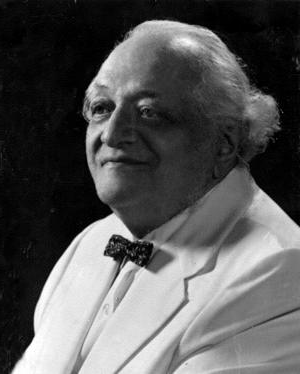
\includegraphics[width=.3\textwidth]{moreno.png}
\end{frame}

\begin{frame}{Sociogram}
\centering
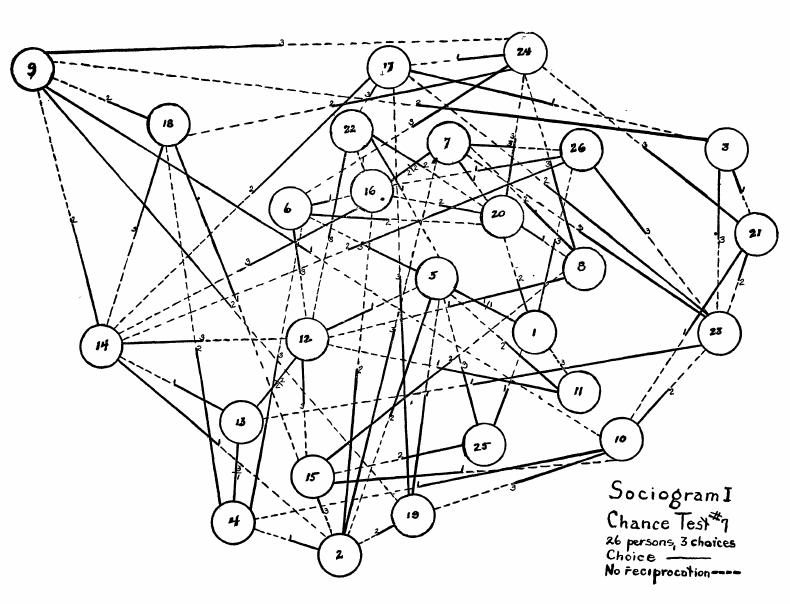
\includegraphics[width=.8\textwidth]{sociogram.png}
\blfootnote{
    Moreno, J. L., \& Jennings, H. H. (1938). Statistics of Social Configurations.
    Sociometry, 1(3/4), 342. https://doi.org/10.2307/2785588
}
\end{frame}

\section{Basic concepts}

\begin{frame}{Graph definition}
\begin{itemize}
    \item<1-> Graph is a 2-tuple $G = (V, E)$ where $V$ is a set of entities
    know as nodes or vertices and $E$ is a set of connections between
    nodes, which are called edges (or links/ties).
    \item<2-> $G$ can be also associated with sets of node or edge attributes.
    \item<3-> A node attribute is a function $f: V \to A$ where $A$ is any
    set of values the attribute may take.
    \item<4-> Similarly, an edge attribute is a function $g: E \to B$ where
    $B$ is an arbitrary set of values.
\end{itemize}
\end{frame}

\begin{frame}{Graph definition | Example}
\begin{columns}
\column{.5\textwidth}
    \begin{center}
    \begin{tikzpicture}[node distance=2cm]
        \node[vertex] (A) {$A$};
        \node[vertex, left of=A] (B) {$B$};
        \node[vertex, fill=red, below of=A] (C) {$C$};
        % Edges
        \path[draw, line width=.5mm]
        (A) -- node[weight] {$1$} (B);
        \path[draw, line width=1mm]
        (A) -- node[weight] {$2$} (C);
    \end{tikzpicture}
    \end{center}
\column{.5\textwidth}
    \begin{itemize}
        \item<2-> $V = \{A, B, C\}$
        \item<3-> $\text{color}: V \to \{\text{\faStop}, \text{\red{\faStop}}\}$
        \item<4-> $E = \{(A, B), (A, C)\}$
        \item<5-> $\text{weight}: E \to \mathbb{R}$
    \end{itemize}
\end{columns}
\end{frame}

\begin{frame}{Remark on weights}
\begin{itemize}
    \item<1-> Networks are often \textbf{weighted} meaning that different edges
    may be of different importance.
    \item<2-> Usually weights indicate strength/closeness of a relationship,
    but in some applications they can also refer to the distance between
    two nodes.
    \item<3-> Due to time constraints we will avoid discussing methods for
    weighted networks almost completely. However, once you know the standard
    unweighted methods it should not be too hard to learn about their
    weighted counterparts.
    \item<4-> However, mathematical details of weighted methods are often
    significantly more involved.
\end{itemize}
\end{frame}

\begin{frame}{Undirected and directed graphs}
\begin{columns}
\column{.5\textwidth}
\begin{center}
    \begin{tikzpicture}[node distance=2cm]
        \node[vertex] (A) {$A$};
        \node[vertex, left of=A] (B) {$B$};
        \node[vertex, below of=A] (C) {$C$};
        % Label
        \node[label, above left of=A] (label) {Undirected};
        % Edges
        \path[draw, ultra thick]
        (A) -- (B)
        (A) -- (C);
    \end{tikzpicture}
    \begin{itemize}
        \item $V = \{A, B, C\}$
        \item $E = \{(A, B), (A, C)\}$
    \end{itemize}
    \end{center}
\pause
\column{.5\textwidth}
\begin{center}
    \begin{tikzpicture}[node distance=2cm]
        \node[vertex] (A) {$A$};
        \node[vertex, left of=A] (B) {$B$};
        \node[vertex, below of=A] (C) {$C$};
        % Label
        \node[label, above left of=A] (label) {Directed};
        % Edges
        \draw[->, edge] (A) -- (B);
        \draw[->, edge] (A) -- (C);
        \draw[->, edge] (C) -- (A);
    \end{tikzpicture}
    \begin{itemize}
        \item $V = \{A, B, C\}$
        \item $E = \{(A, B), (A, C), (C, A)\}$
    \end{itemize}
\end{center}
\end{columns}
\end{frame}

\begin{frame}{Matrix representation}
\begin{columns}
\column{.5\textwidth}
\begin{center}
    \begin{tikzpicture}[node distance=2cm]
        \node[vertex] (A) {$A$};
        \node[vertex, left of=A] (B) {$B$};
        \node[vertex, below of=A] (C) {$C$};
        % Edges
        \path[draw, ultra thick]
        (A) -- (B)
        (A) -- (C);
    \end{tikzpicture}
    \end{center}
\pause
\column{.5\textwidth}
\begin{center}
    \[
        \mathbf{A} =
        \begin{array}{c|ccc}
            & A & B & C \\
            \hline
          A & 0 & 1 & 1 \\
          B & 1 & 0 & 0 \\
          C & 1 & 0 & 0
        \end{array}
    \]
\end{center}
\end{columns}
\end{frame}

\begin{frame}{Adjacency matrix}
\begin{itemize}
    \item<1-> Adjacency matrix may seem a bit redundant when compared
    to a simple edge list.
    \item<2-> However, this representation allows applying powerful tools
    of matrix algebra to graphs and is really the foundation of many useful
    methods.
    \item<3-> But it requires somewhat more advanced mathematical training
    (i.e. knowledge of matrix/linear algebra), so we will discuss only one
    simple application later on.
\end{itemize}
\end{frame}

\begin{frame}{Edge density}
\begin{itemize}
    \item<2-> How many edges are possible in a \textbf{directed network}
        with $N$ nodes?
    \begin{itemize}
        \item<3-> $N(N-1)$
    \end{itemize}
    \item<4-> How many edges are possible in an \textbf{undirected network}
    with $N$ nodes?
    \begin{itemize}
        \item<5-> $\frac{N(N-1)}{2}$
    \end{itemize}
    \item<6-> Edge density is defined simply as:
    \[
        \frac{\text{\# of edges}}{\text{\# of possible edges}}
    \]
\end{itemize}
\end{frame}

\begin{frame}{Network walks}
\begin{itemize}
    \item A walk on a network is any sequence along
    multiple connected nodes.
\end{itemize}
\pause
\begin{center}
\begin{tikzpicture}[node distance=1.5cm]
    \node[vertex] (A) {$A$};
    \node[vertex, left of=A] (B) {$B$};
    \node[vertex, below of=A] (C) {$C$};
    \node[vertex, right of=A] (D) {$D$};
    \node[vertex, above right of=A] (E) {$E$};
    % Edges
    \draw[edge] (A) -- (B);
    \draw[edge] (A) -- (C);
    \draw[edge] (C) -- (A);
    \draw[edge] (A) -- (D);
    \draw[edge] (A) -- (E);
    \draw[edge] (D) -- (E);
\end{tikzpicture}
\end{center}
\begin{itemize}
    \item<3-> For instance, $C-A-D-E-A-B$ is a walk.
    \item<4-> Note that above $A$ occurred two times within the walk.
\end{itemize}
\end{frame}

\begin{frame}{Network paths}
\begin{itemize}
    \item A path on a network is any sequence along multiple
    connected nodes in which each node is used \textbf{only once}.
\end{itemize}
\pause
\begin{center}
\begin{tikzpicture}[node distance=1.5cm]
    \node[vertex] (A) {$A$};
    \node[vertex, left of=A] (B) {$B$};
    \node[vertex, below of=A] (C) {$C$};
    \node[vertex, right of=A] (D) {$D$};
    \node[vertex, above right of=A] (E) {$E$};
    % Edges
    \draw[edge] (A) -- (B);
    \draw[edge] (A) -- (C);
    \draw[edge] (C) -- (A);
    \draw[edge] (A) -- (D);
    \draw[edge] (A) -- (E);
    \draw[edge] (D) -- (E);
\end{tikzpicture}
\end{center}
\begin{itemize}
    \item<3-> For instance, $D-E-A-B$ is a path.
    \item<4-> But $C-A-D-E-A-B$ is not a path.
\end{itemize}
\end{frame}

\begin{frame}{Node degree}
\begin{itemize}
    \item<2-> Perhaps the most important property of each node is its \textbf{degree}.
    \item<3-> The degree of a node $i$, often denoted by $d_i$ or $k_i$,
    is equal to the number of other nodes it is linked to.
    \pause
    \begin{center}
    \begin{tikzpicture}[node distance=1.5cm]
        \node[vertex] (A) {$A$};
        \node[vertex, left of=A] (B) {$B$};
        \node[vertex, below of=A] (C) {$C$};
        \node[vertex, right of=A] (D) {$D$};
        \node[vertex, above right of=A] (E) {$E$};
        % Edges
        \draw[edge] (A) -- (B);
        \draw[edge] (A) -- (C);
        \draw[edge] (C) -- (A);
        \draw[edge] (A) -- (D);
        \draw[edge] (A) -- (E);
        \draw[edge] (D) -- (E);
    \end{tikzpicture}
    \end{center}
    \begin{itemize}
        \item<5-> For instance, here $d_C = 1$.
    \end{itemize}
\end{itemize}
\end{frame}

\begin{frame}{Node degree as a centrality measure}
\begin{itemize}
    \item<2-> \textbf{Node degree} is the most basic but also arguably most
    fundamental \textbf{centrality measure}.
    \item<3-> It is a \textbf{first-order measure} as it account only for the
    \textbf{local environment} of a node.
    \item<4-> Centrality measures tell us which nodes are most important
    from the vantage point of the connectivity of a network.
    \item<5-> There are many different centrality measures focused on different
    aspects of the overall structure and later on we will discuss one more
    very important measure of a much more global character.
\end{itemize}
\end{frame}

\begin{frame}{Node degrees in directed graphs}
\begin{itemize}
    \item<2-> In directed graphs one need to consider both in-degrees
    and out-degrees (and total degrees which are their sums).
\end{itemize}
\pause
\begin{center}
\begin{tikzpicture}[node distance=1.5cm]
    \node[vertex] (A) {$A$};
    \node[vertex, below left of=A] (B) {$B$};
    \node[vertex, below right of=A] (C) {$C$};
    \node[vertex, right of=C] (D) {$D$};
    % Edges
    \draw[->, edge] (A) -- (B);
    \draw[->, edge] (A) -- (C);
    \draw[->, edge] (C) -- (D);
\end{tikzpicture}
\end{center}
\pause
\begin{itemize}
    \item Both in-degree and out-degree of $C$ are equal to $1$.
    What are degrees of other nodes?
\end{itemize}
\end{frame}

\begin{frame}{Connectedness \& components}
\begin{itemize}
    \item The network below is not connected and consists of three
    components of which one is a single isolated node (isolate).
\end{itemize}
\begin{center}
\begin{tikzpicture}[node distance=1.5cm]
    \node[vertex] (A) {$A$};
    \node[vertex, below left of=A] (B) {$B$};
    \node[vertex, below right of=A] (C) {$C$};
    \node[vertex, right of=C] (D) {$D$};
    \node[vertex, right of=D] (E) {$E$};
    \node[vertex, above of=E] (F) {$F$};
    % Edges
    \draw[edge] (A) -- (B);
    \draw[edge] (A) -- (C);
    \draw[edge] (D) -- (E);
\end{tikzpicture}
\end{center}
\pause
\begin{itemize}
    \item Connectedness means that there is a path from any node to
    any other node.
\end{itemize}
\end{frame}

\begin{frame}{Connectedness in directed networks}
\begin{itemize}
    \item<2-> In directed networks there are two notions: \textbf{weak} and
    \textbf{strong} connectedness (and components).
    \item<3-> Weakly connected components are such that are connected
    if directionality of edges is ignored.
    \item<4-> Strongly connected components are such that are connected
    even when directionality of edges is accounted for.
\end{itemize}
\end{frame}

\begin{frame}{Connectedness and random walks on networks}
\begin{itemize}
    \item<1-> Random walk (on a network) is a process in which one starts
    at an arbitrary node and then moves from there to a randomly selected
    neighbour.
    \item<2-> And repeats this process for any number of steps.
\end{itemize}
\end{frame}

\begin{frame}{Random walk on a strongly connected network}
    \animategraphics[
        autoplay,
        loop,
        width=.9\textwidth
    ]{3}{overview/rw-strong/rw_strong-}{1}{8}
\end{frame}

\begin{frame}{Random walk on a weakly connected network}
    \animategraphics[
        autoplay,
        loop,
        width=.9\textwidth
    ]{3}{overview/rw-weak/rw_weak-}{1}{24}
\end{frame}

\begin{frame}{Bipartite graphs}
\begin{itemize}
    \item<1-> In many applications including elite studies based on so-called
    affiliation networks one finds bipartite graphs.
    \item<2-> A bipartite graph is composed of two distinct types of entities
    (nodes) and connections are allowed only between different types.
    \item<3-> For instance, one can consider an affiliation network composed
    of high managers and companies they worked in.
\end{itemize}
\end{frame}

\begin{frame}{Bipartite graph | Example}
\begin{center}
\begin{tikzpicture}[node distance=2.5cm]
    \node[vertex] (Jane) {Jane};
    \node[vertex, right of=Jane] (Adam) {Adam};
    \node[vertex, color=black, fill=white, above of=Jane] (Google) {Google};
    \node[vertex, color=black, fill=white, right of=Google] (Shell) {Shell};
    % Edges
    \draw[edge] (Jane) -- (Google);
    \draw[edge] (Jane) -- (Shell);
    \draw[edge] (Adam) -- (Shell);
\end{tikzpicture}
\end{center}
\end{frame}

\section{Generative model \& random graphs}

\begin{frame}{Generative models | ER random graph}
\begin{itemize}
    \item<1-> One of the central questions in network science is what are possible
    \textbf{generating processes} that may produce particular kinds of networks.
    \item<2-> The first and foremost model proposed already in 1959 by two
    famous Hungarian mathematicians --- Paul Erdős and Alfréd Rényi ---
    is know as \textbf{Erdős-Rényi model} or \textbf{ER random graph model}.
    \item<3-> It is controlled by two parameters, $N$ and $p$, where $N$
    specifies the number of nodes and $p$ is the probability that any two nodes
    are connected.
\end{itemize}
\end{frame}

\begin{frame}{ER random graph | Example}
\begin{columns}
\column{.5\textwidth}
    \centering
    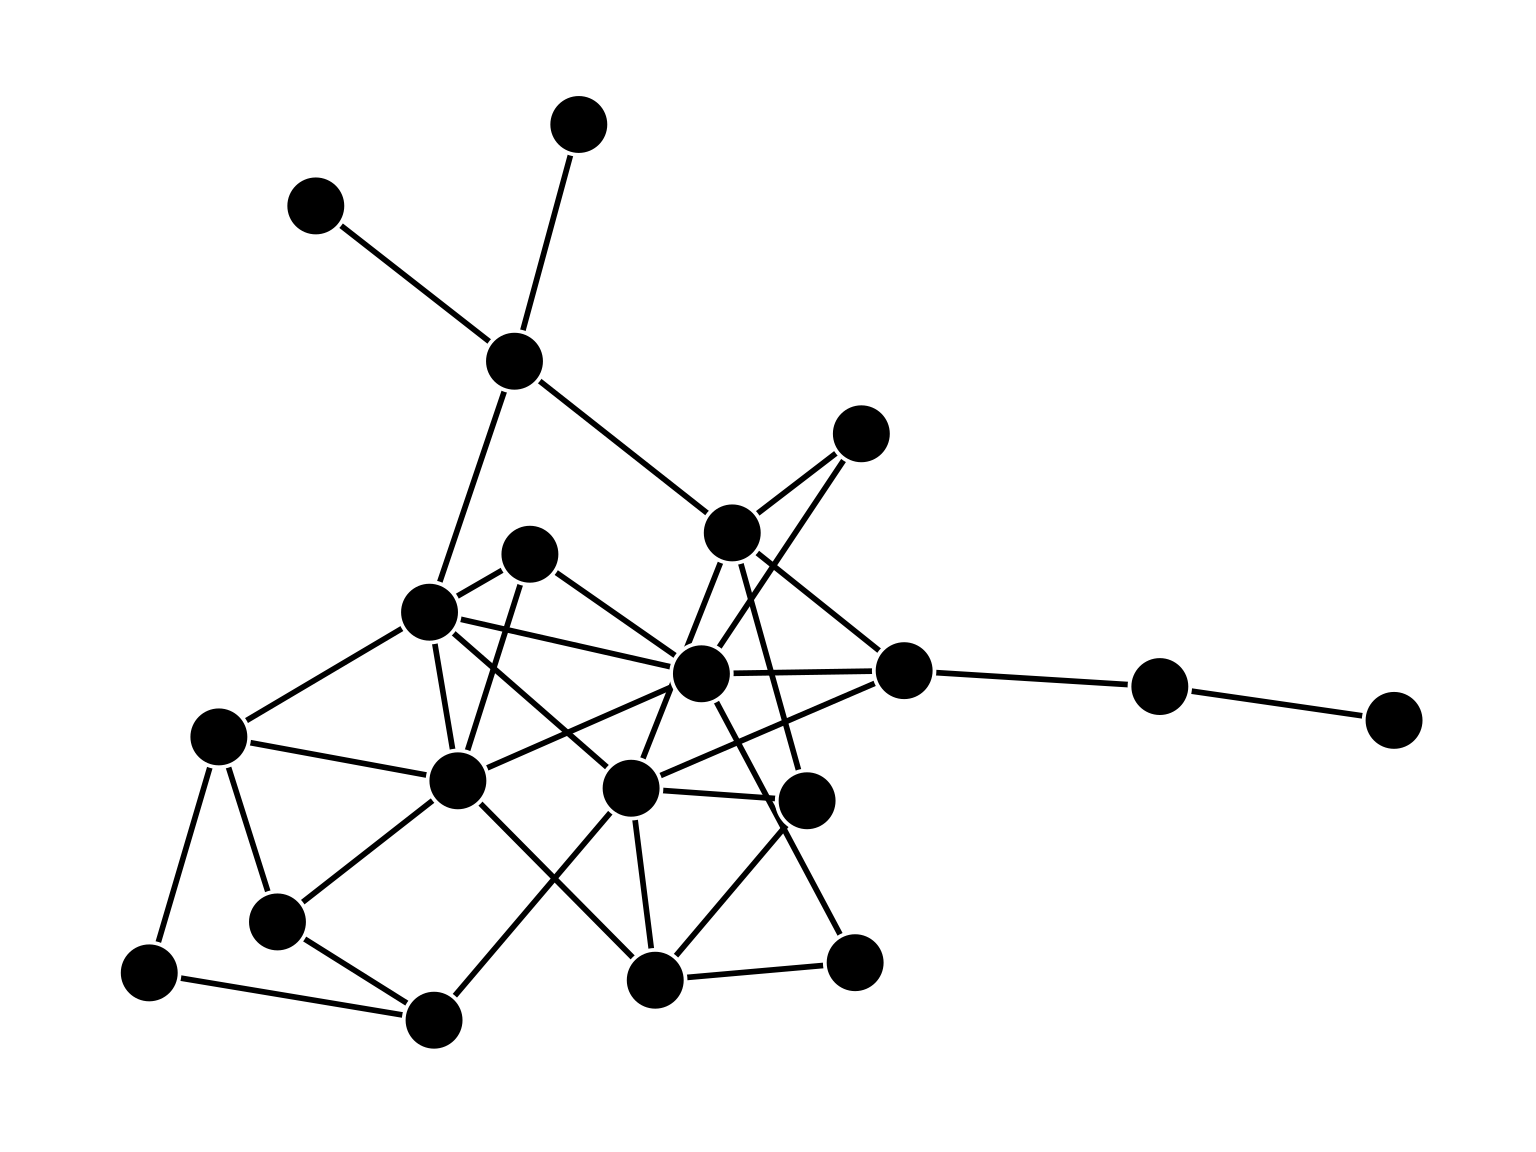
\includegraphics[width=\textwidth]{overview/er_random_graph-1.png}
\column{.5\textwidth}
    \centering
    \[
        \begin{pmatrix}
             & \gray{p} & \gray{p} & \gray{p} \\
            p &  & \gray{p} & \gray{p} \\
            p & p &  & \gray{p} \\
            p & p & p &  \\
        \end{pmatrix}
    \]
\end{columns}
\end{frame}

\begin{frame}{ER random graph is usually not realistic}
\begin{itemize}
    \item<1-> Once people started to analyze real-world networks they quickly
    realized that ER random graph model does not reproduce many of their
    typical features.
    \item<2-> We will spend quite some time in this class trying to figure
    out what are the typical properties of social networks.
    \item<3-> For now, we will focus on one of the properties ER model captures
    surprisingly well.
\end{itemize}
\end{frame}

\begin{frame}{Edge density in ER model}
\begin{itemize}
    \item<2-> In ER model $p$ specifies the probability that any edge exists.
    \item<3-> And in an undirected networks we have $N(N-1)/2$ possible
    edges.
    \item<4-> Let $X_{ij}$ be a random variable corresponding to potential
    edge between nodes $i$ and $j$.
    \item<5-> So expected edge density under ER model is:
    \[
        \E\left[
            \sum_{i, j < i}\frac{X_{ij}}{N(N-1)/2}
        \right]
        =
        \frac{\sum_{i, j<i}\E[X_{ij}]}{N(N-1)/2}
        =
        \frac{pN(N-1)/2}{N(N-1)/2}
        =
        p
    \]
\end{itemize}
\end{frame}

\begin{frame}{Edge density in ER model}
\begin{itemize}
    \item<2-> So in ER model we can use $p$ parameter to reproduce any edge
    density we want (on average).
    \item<3-> But the model fails to reproduce most other properties.
    \item<4-> Except for one other important property, which we will discuss later.
\end{itemize}
\end{frame}

\begin{frame}{Degree distribution in ER model}
\begin{itemize}
    \item<2-> Before sampling each edge is a Bernoulli random variable
    (i.e. it is $1$ with probability $p$ or $0$ otherwise):
    \[
        \begin{pmatrix}
             & \gray{X_{12}} & \gray{X_{13}} & \gray{X_{14}} \\
            X_{21} &  & \gray{X_{23}} & \gray{X_{24}} \\
            X_{31} & X_{32} &  & \gray{X_{34}} \\
            X_{41} & X_{42} & X_{43} &  \\
        \end{pmatrix}
    \]
    \item<3-> Hence, degree of node $i$ is equal to the sum $\sum_{j \neq i}X_{ij}$.
    \item<4-> And we know from basic probability theory that this gives binomial
    distribution with parameters $N-1$ and $p$.
    \item<5-> And for large $N$ converges to Poisson distribution.
\end{itemize}
\end{frame}

\begin{frame}{Degee distribution in ER model is Poissonian!}
\centering
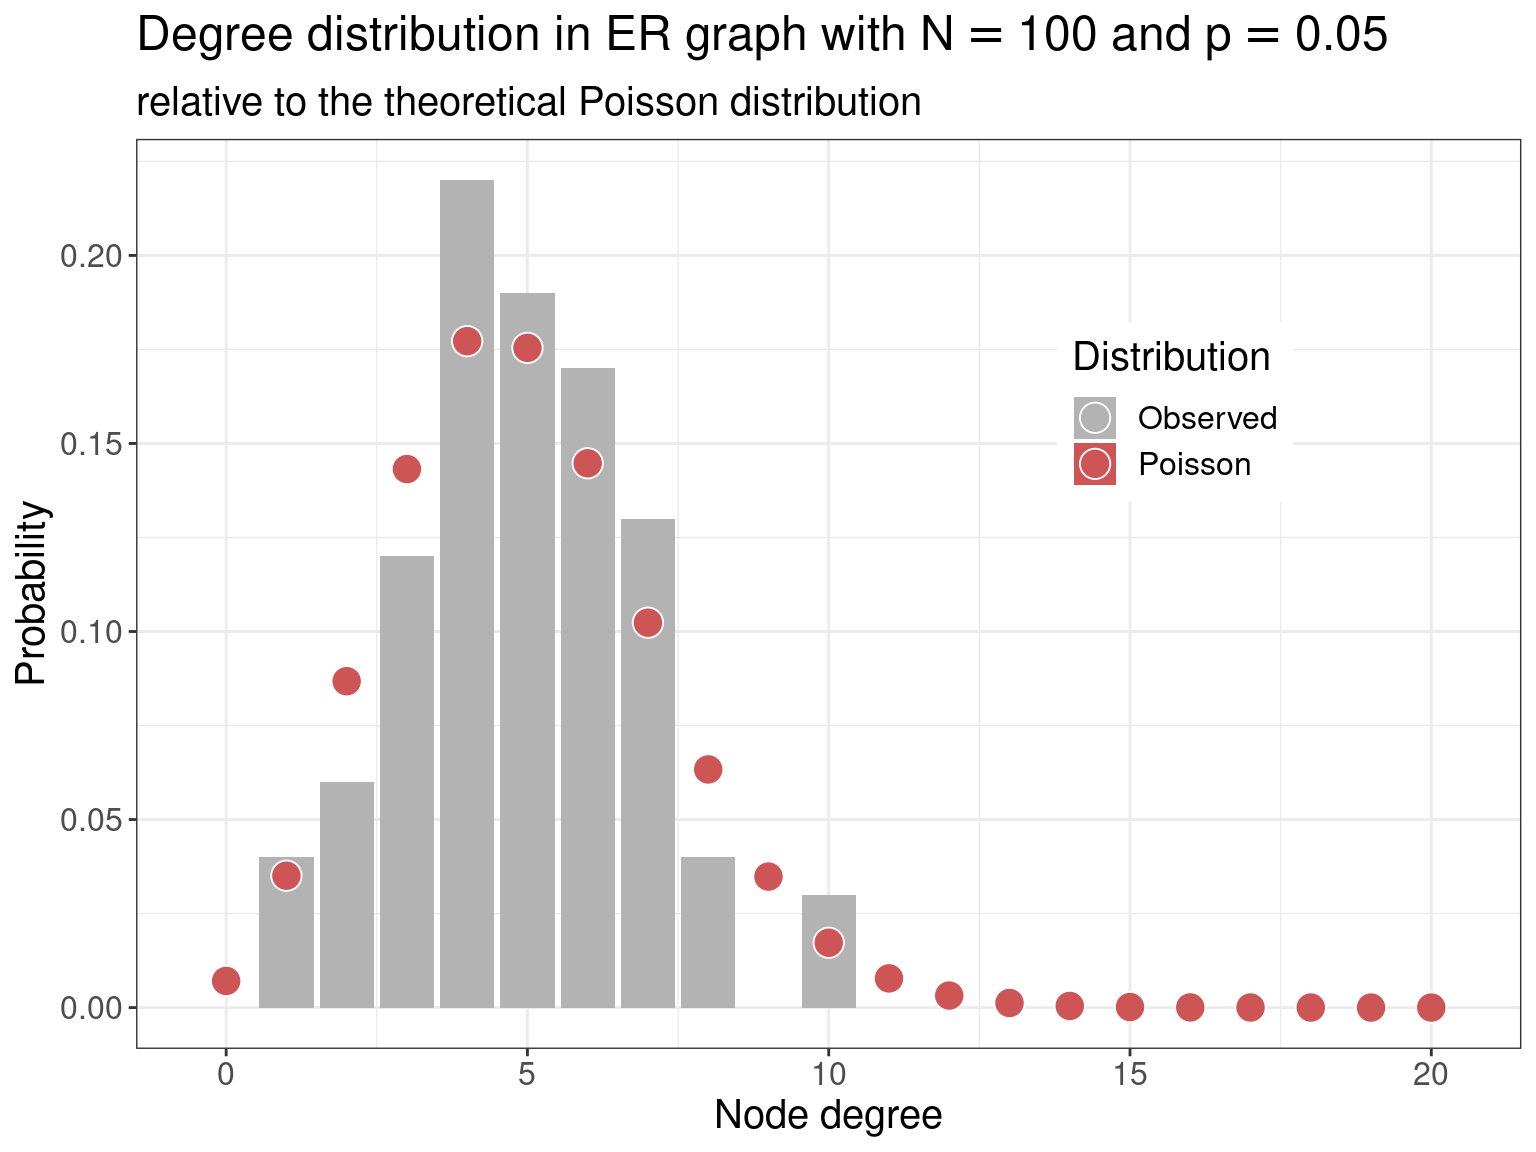
\includegraphics[width=.8\textwidth]{overview/er-poisson-1}
\end{frame}

\begin{frame}{Why are most networks connected?}
\begin{itemize}
    \item<1-> Most real-world networks are roughly connected.
    \item<2-> That is, lion share of nodes almost always belong to
    the so-called \textbf{giant component} (the largest component).
    \item<3-> Why is it so?
    \item<4-> One of the first fundamental results of network science
    was the discovery that this follows directly from ER model.
\end{itemize}
\end{frame}

\begin{frame}{Giant component percolation in ER model | $N = 100, p = .005$}
\centering
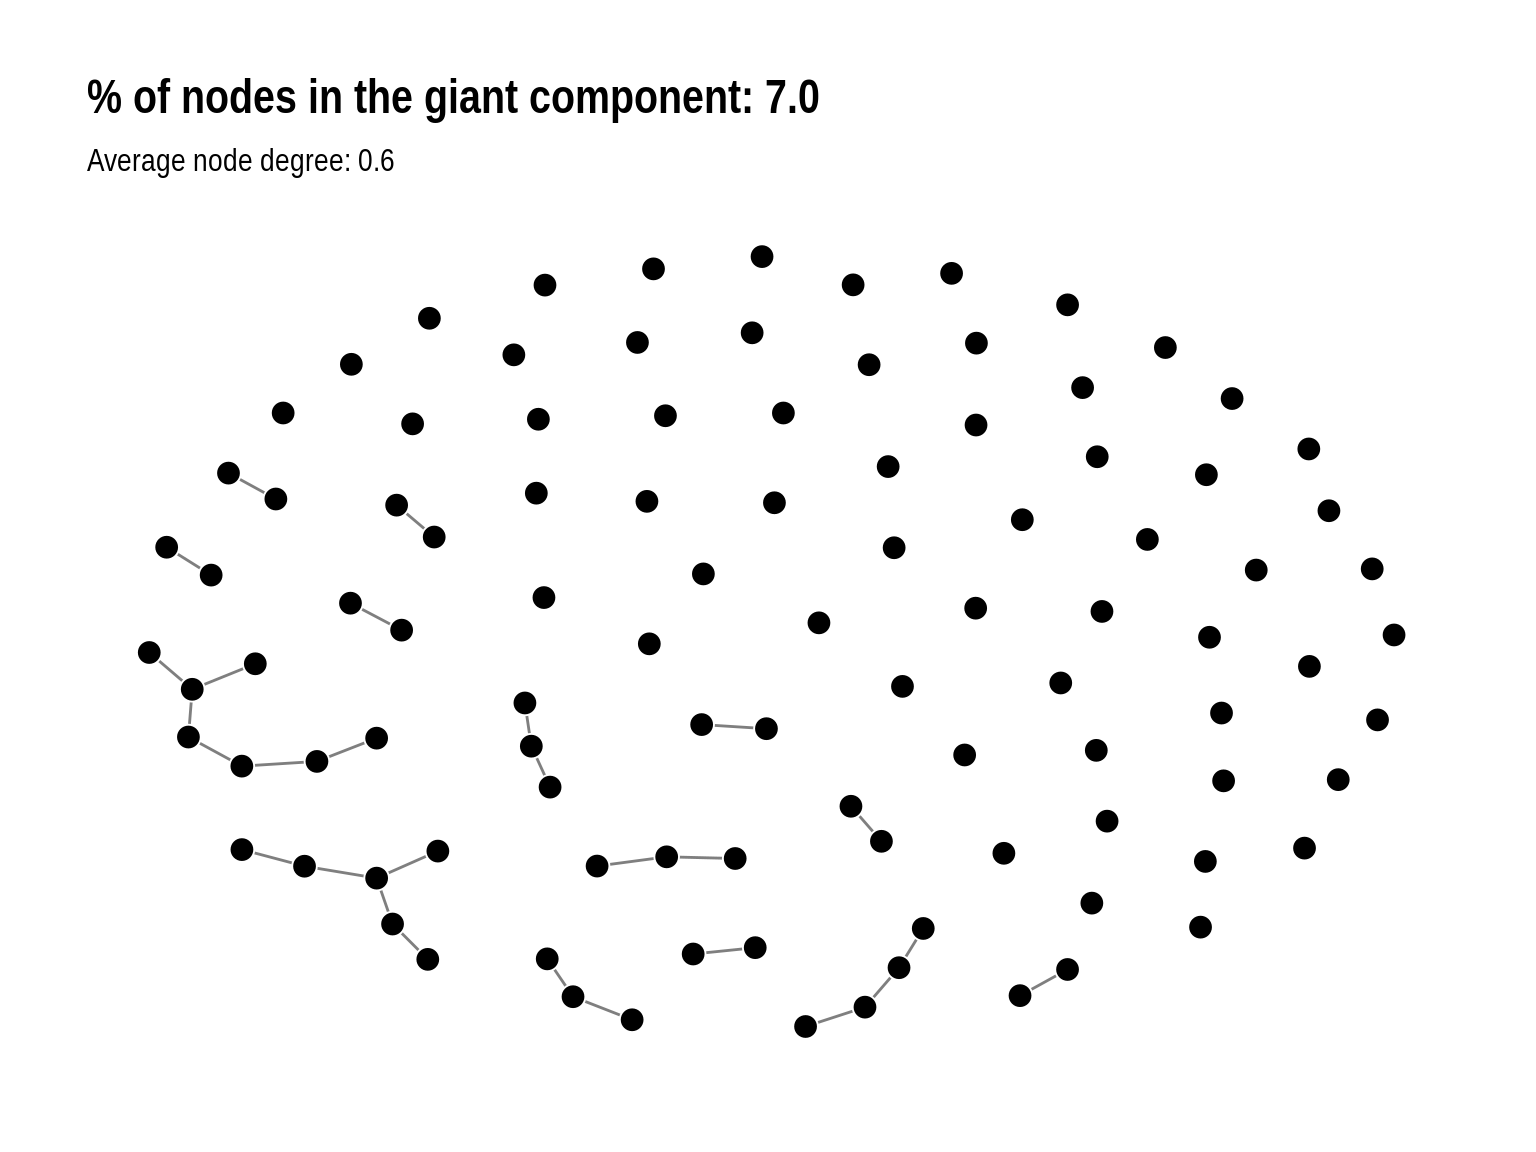
\includegraphics[width=.9\textwidth]{overview/er_model_percolation-1.png}
\end{frame}

\begin{frame}{Giant component percolation in ER model | $N = 100, p = .01$}
\centering
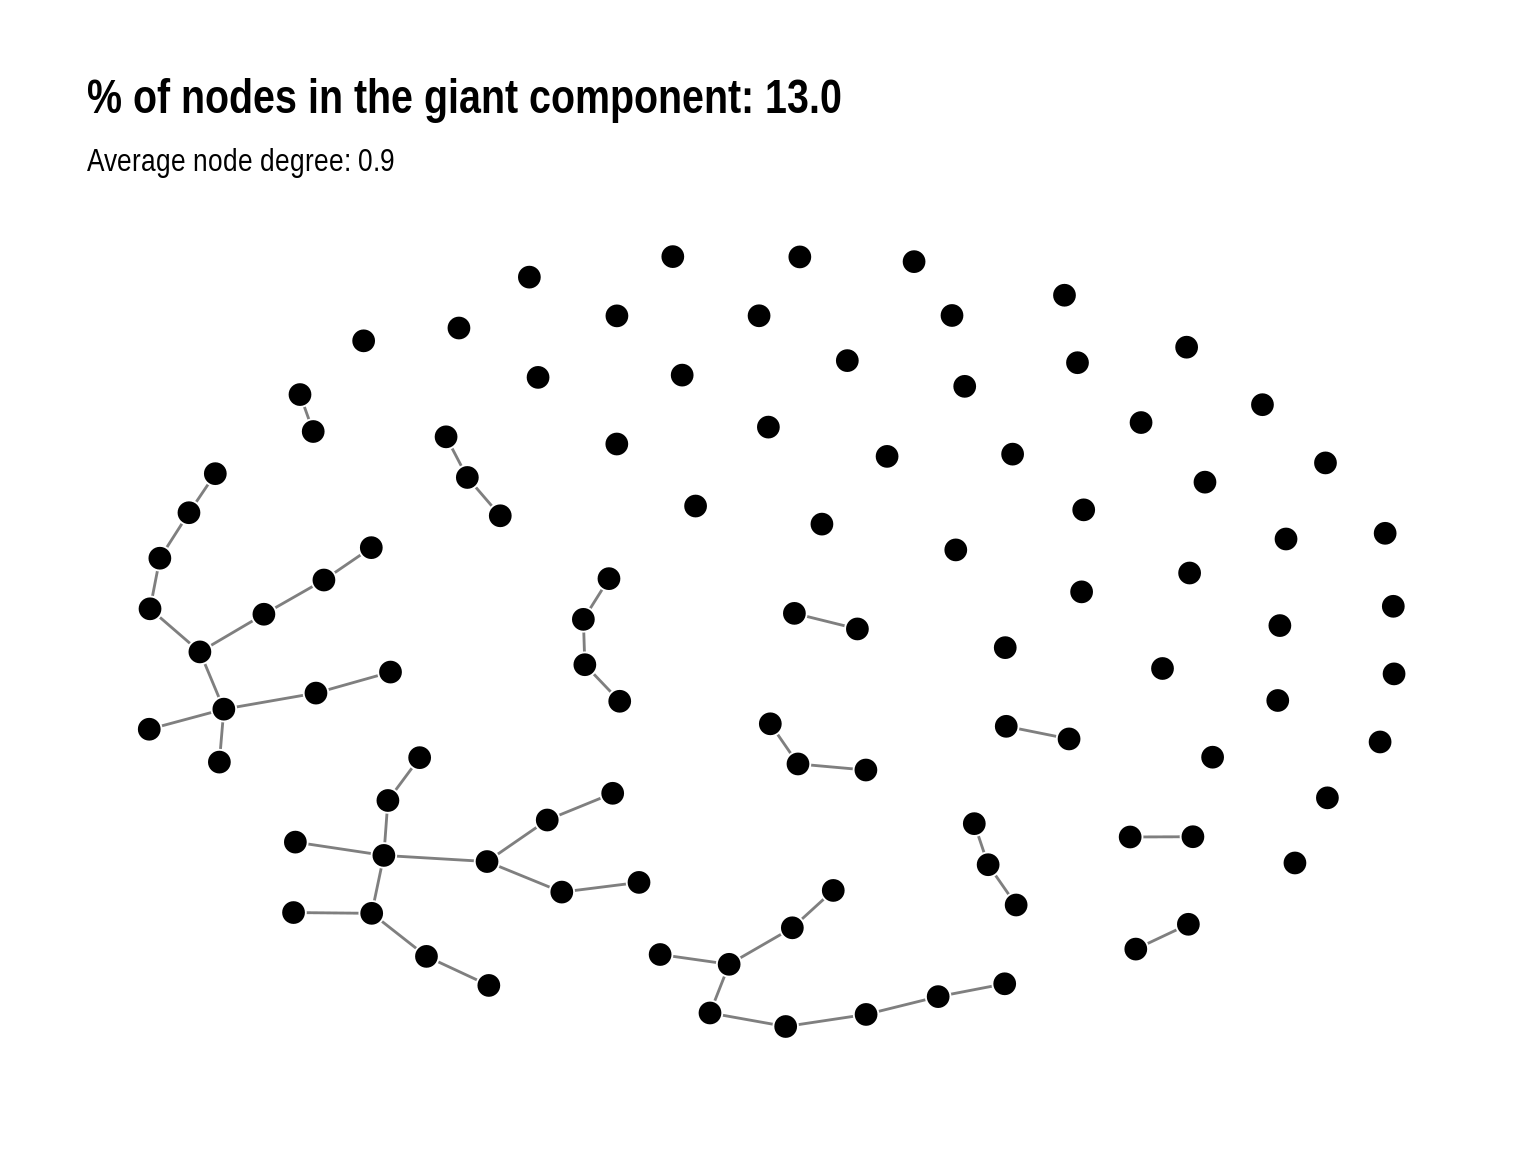
\includegraphics[width=.9\textwidth]{overview/er_model_percolation-2.png}
\end{frame}

\begin{frame}{Giant component percolation in ER model | $N = 100, p = .015$}
\centering
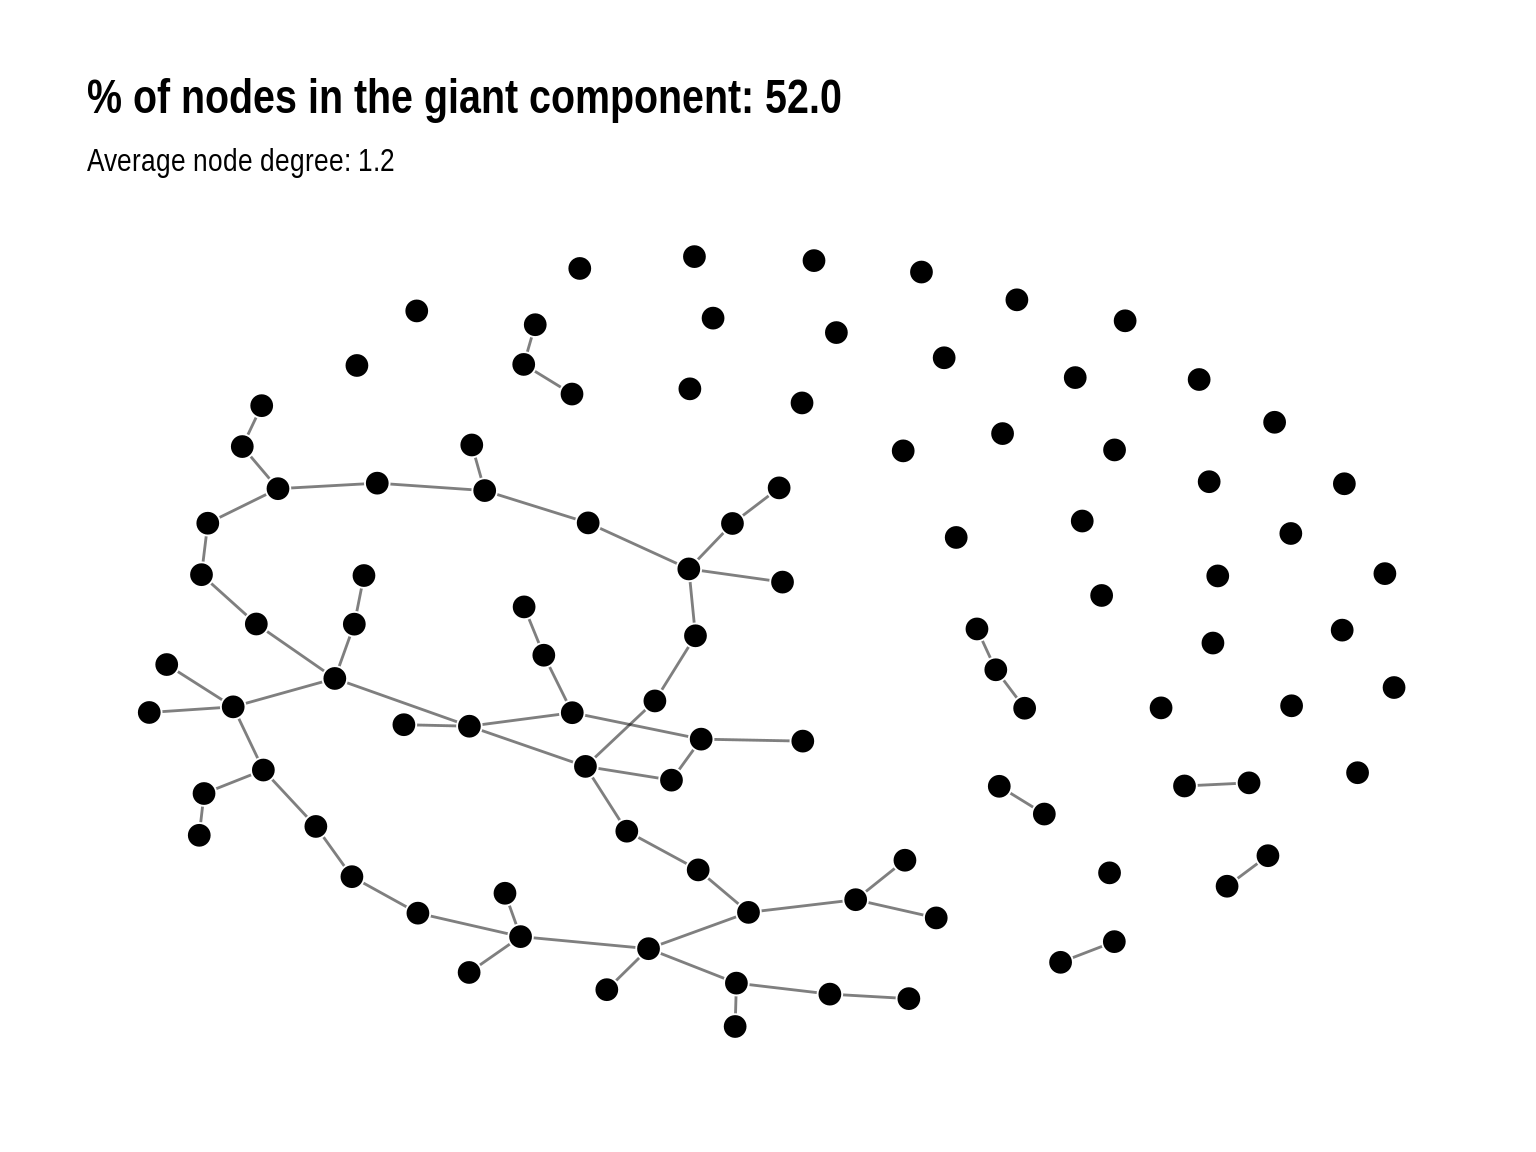
\includegraphics[width=.9\textwidth]{overview/er_model_percolation-3.png}
\end{frame}

\begin{frame}{Giant component percolation in ER model | $N = 100, p = .02$}
\centering
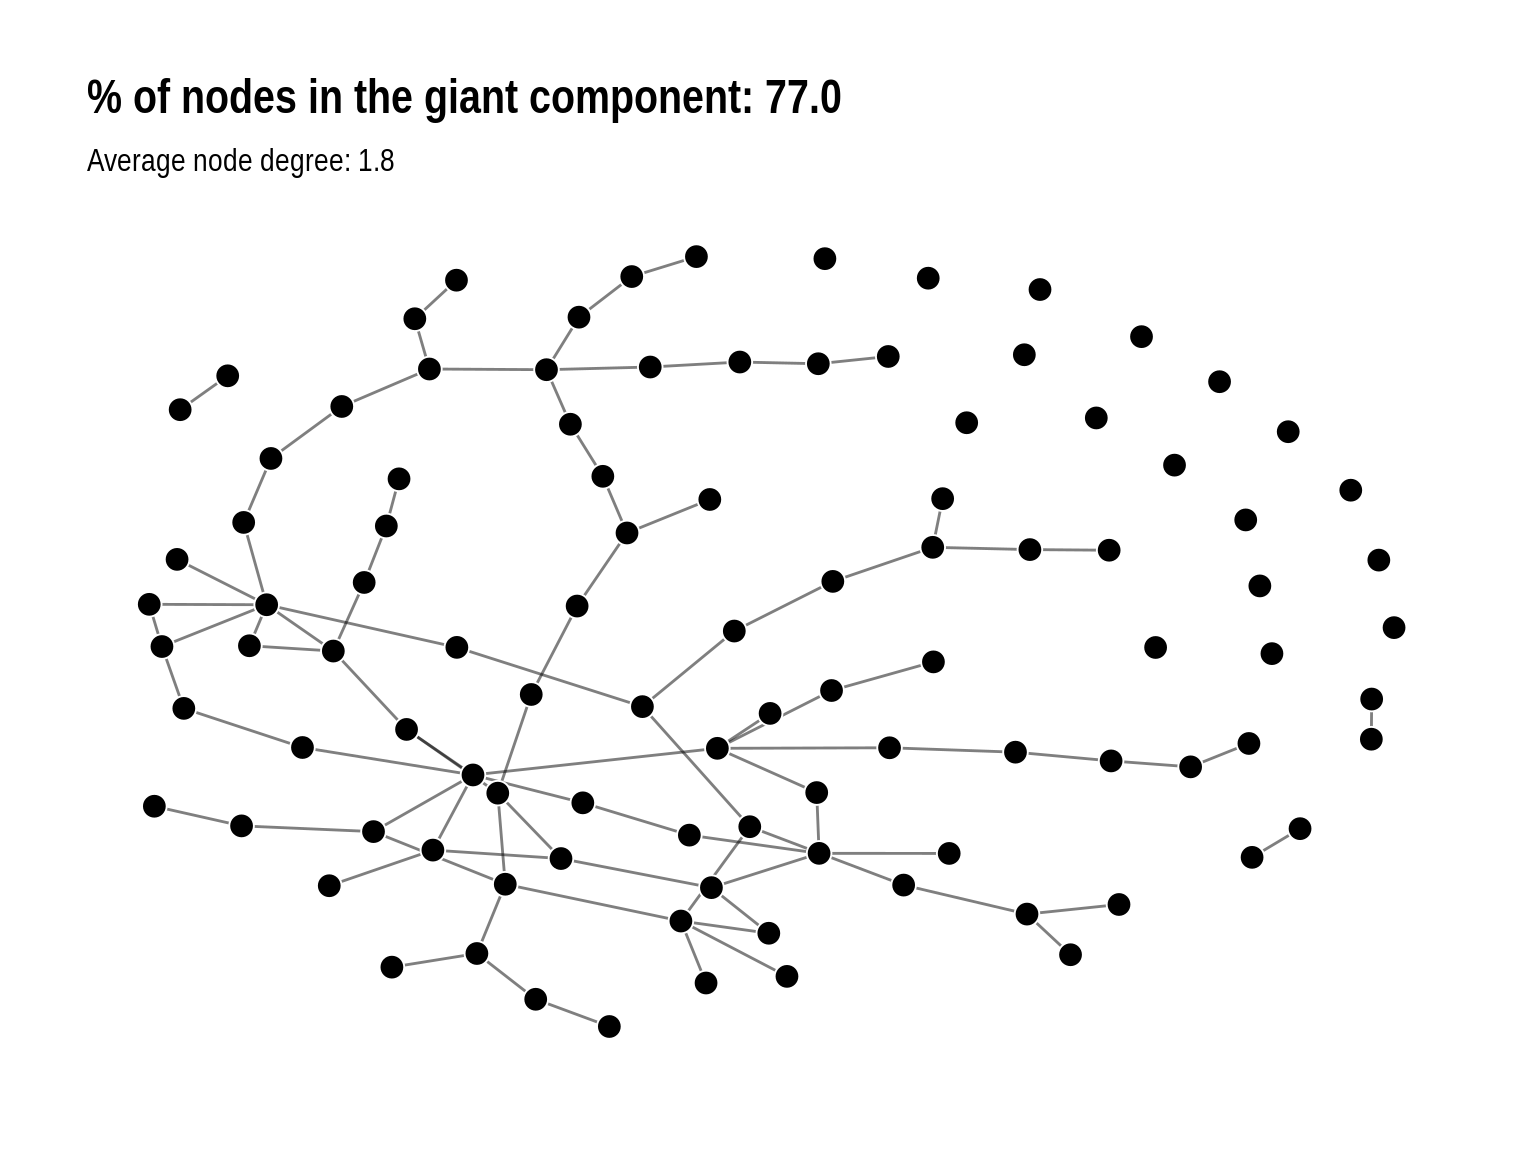
\includegraphics[width=.9\textwidth]{overview/er_model_percolation-4.png}
\end{frame}

\begin{frame}{Giant component percolation in ER model | $N = 100, p = .03$}
\centering
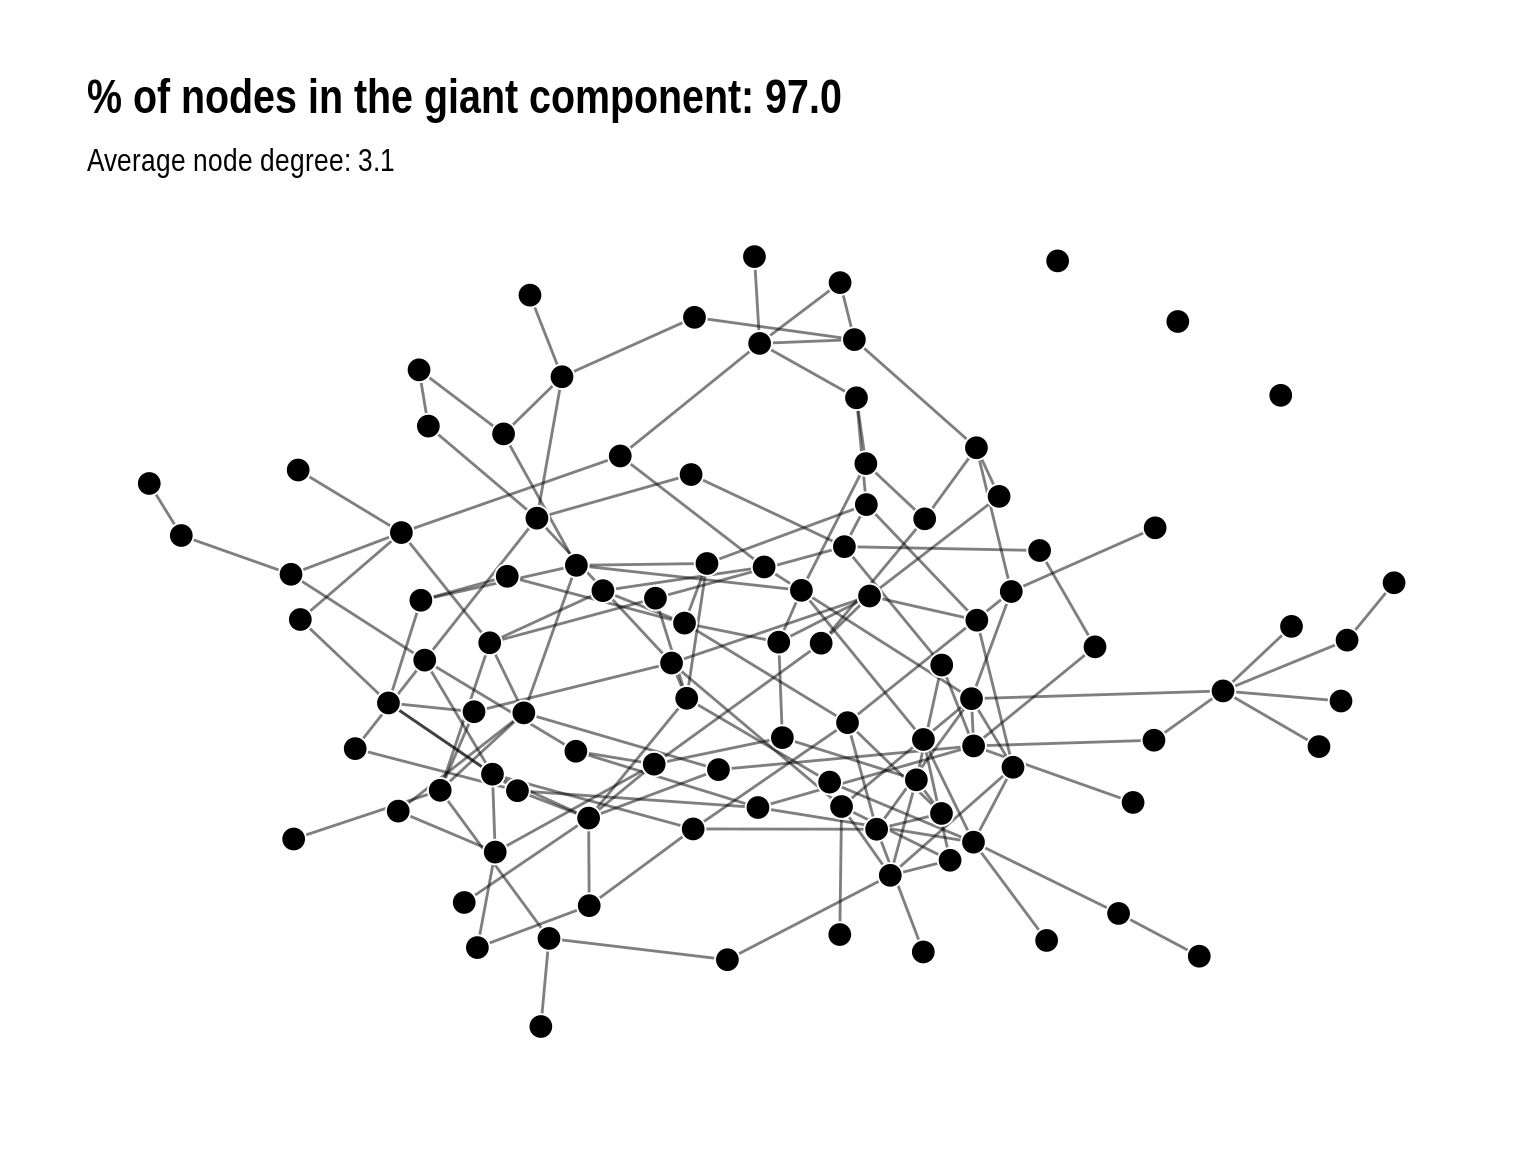
\includegraphics[width=.9\textwidth]{overview/er_model_percolation-5.png}
\end{frame}

\begin{frame}{Giant component percolation in ER model | $N = 100, p = .05$}
\centering
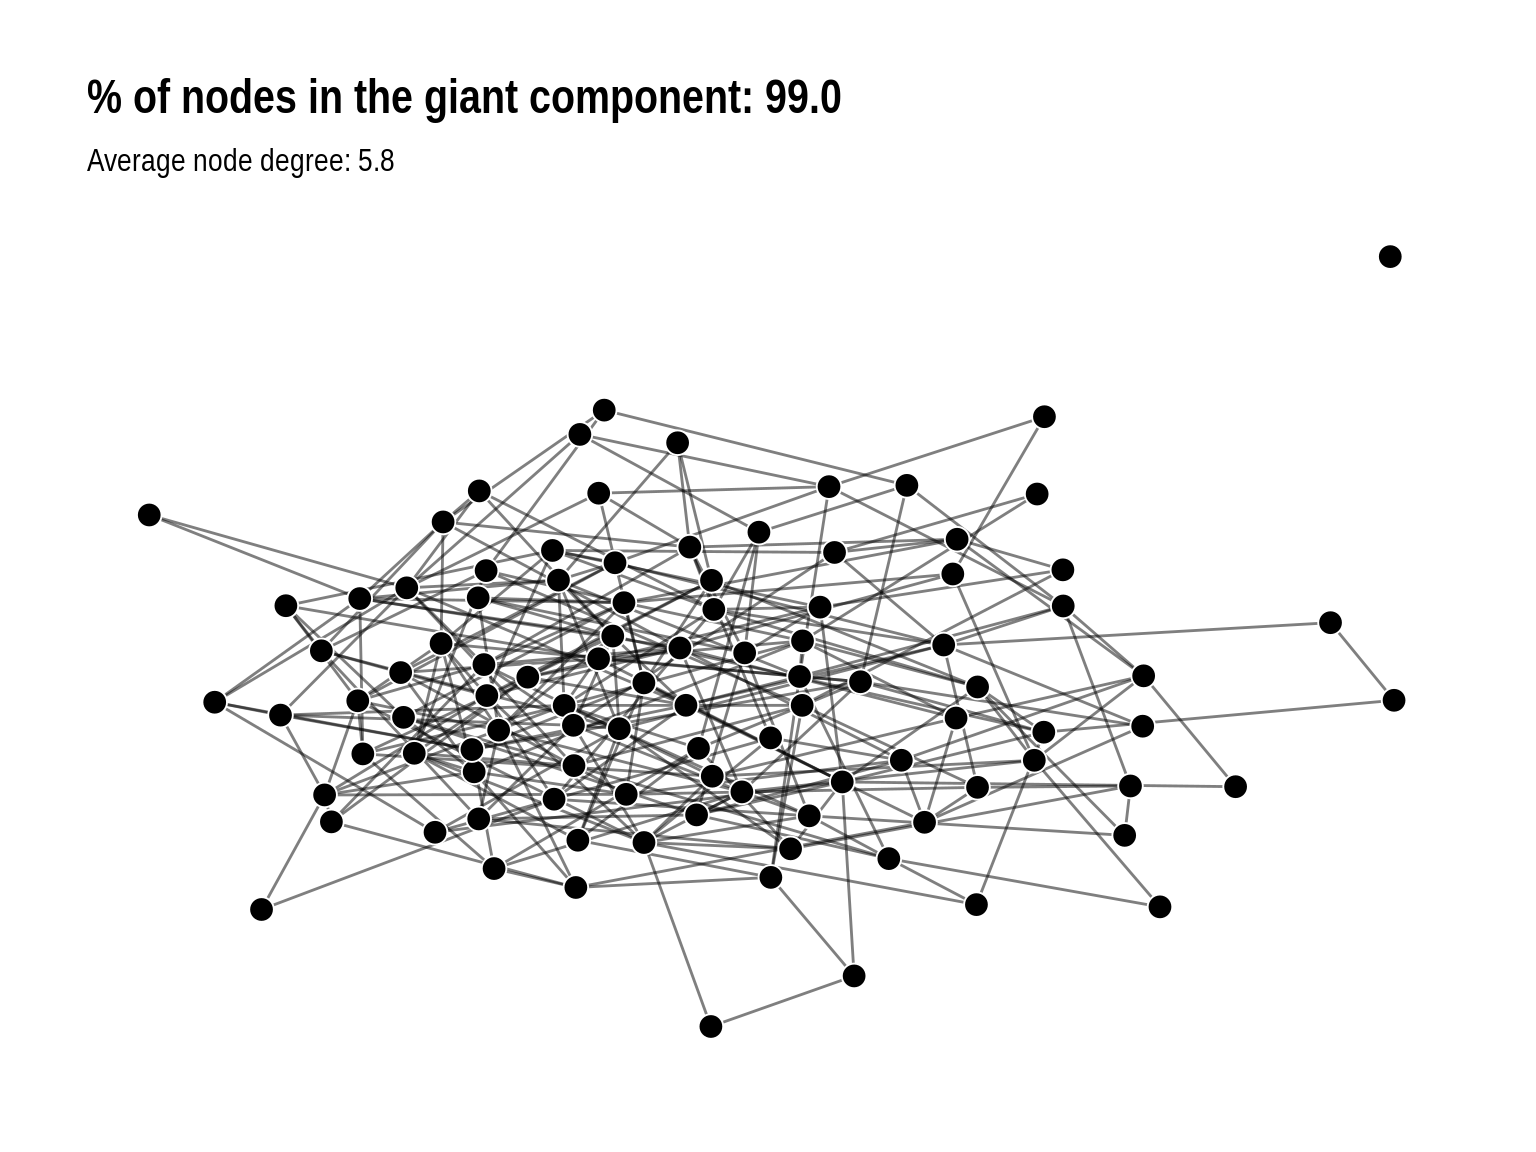
\includegraphics[width=.9\textwidth]{overview/er_model_percolation-6.png}
\end{frame}

\section{Datasets}

\begin{frame}{Hyperlinks between US political blogs (2004)}
\centering
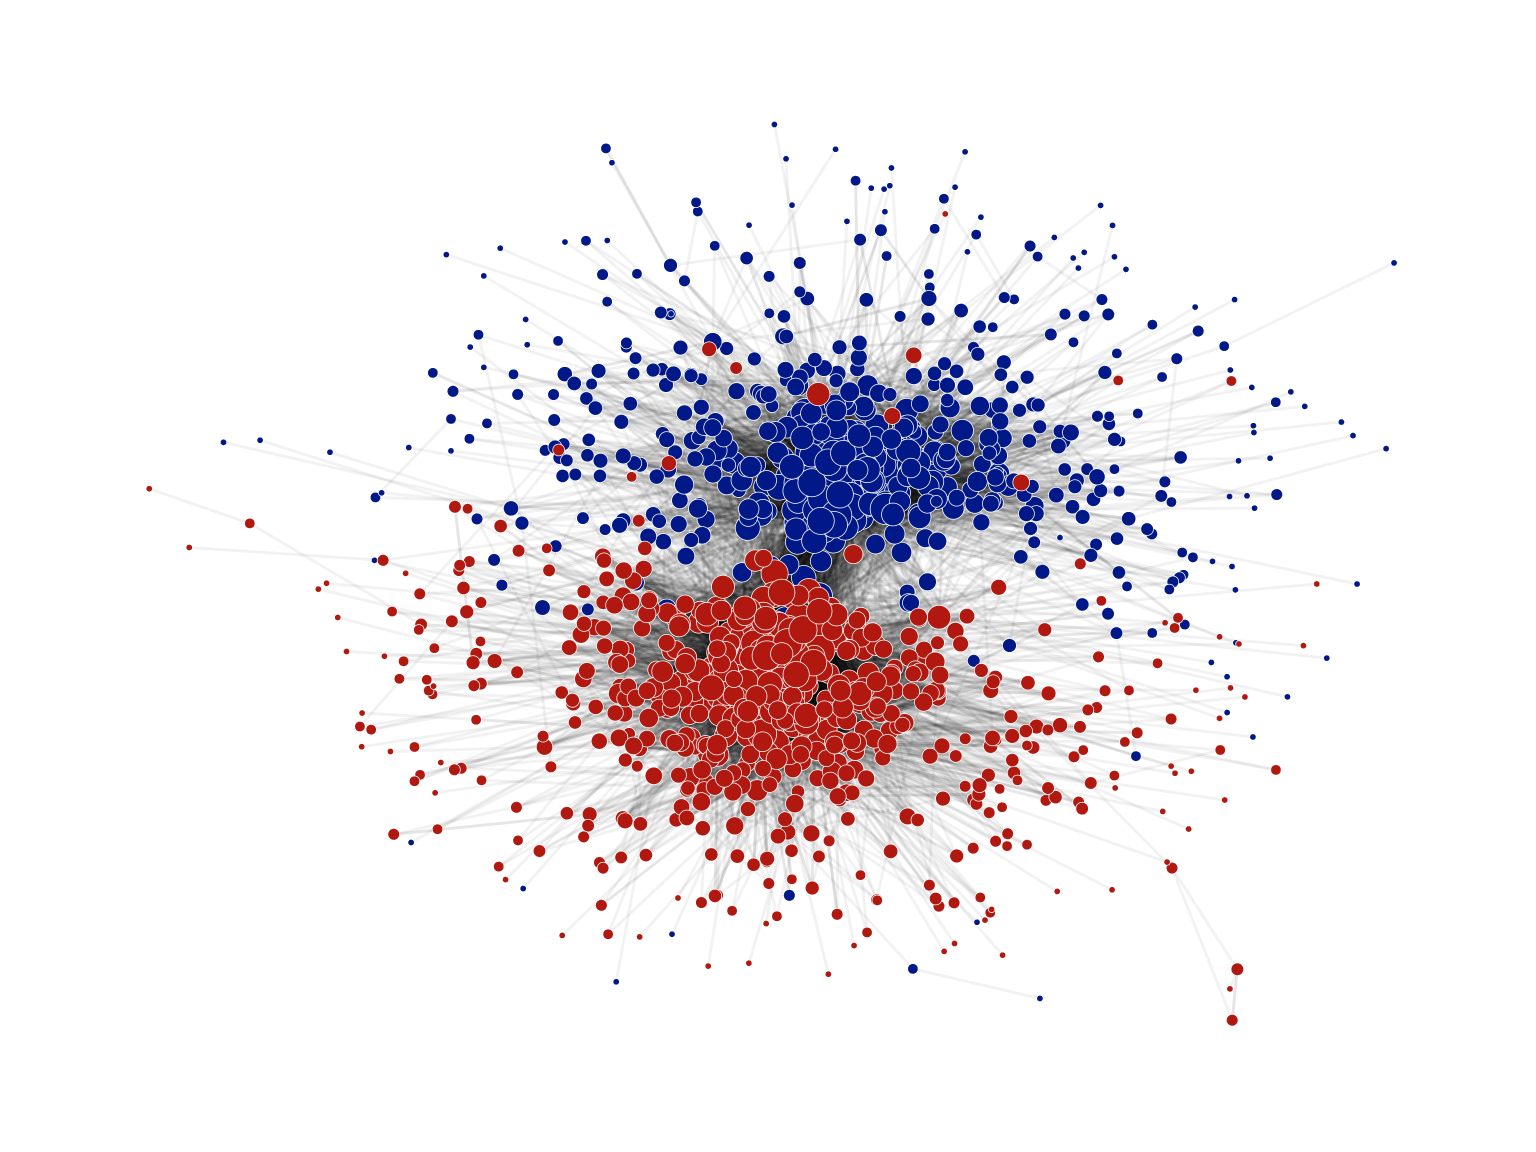
\includegraphics[width=.9\textwidth]{overview/polblogs-1}
\end{frame}

\begin{frame}{Conflict-induced decomposition of a karate club in 1970's (US)}
\centering
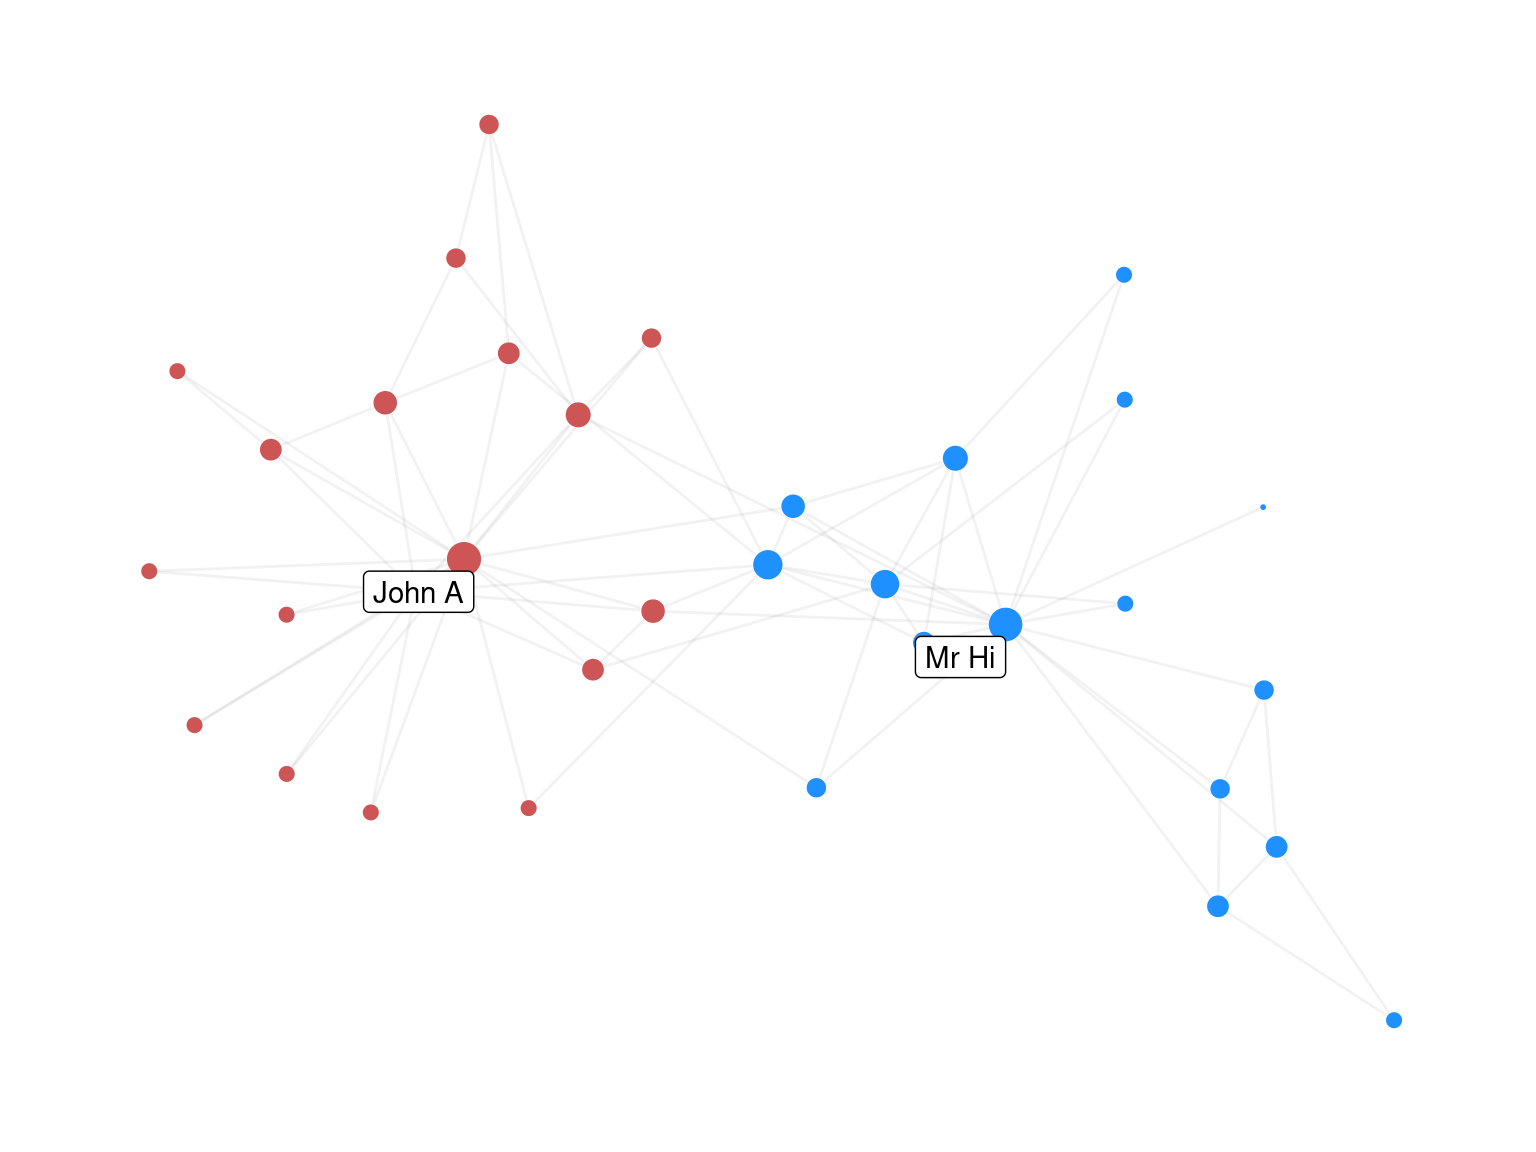
\includegraphics[width=.9\textwidth]{overview/karate-1}
\end{frame}

\begin{frame}{Association within Mexican political elites in XX century}
\centering
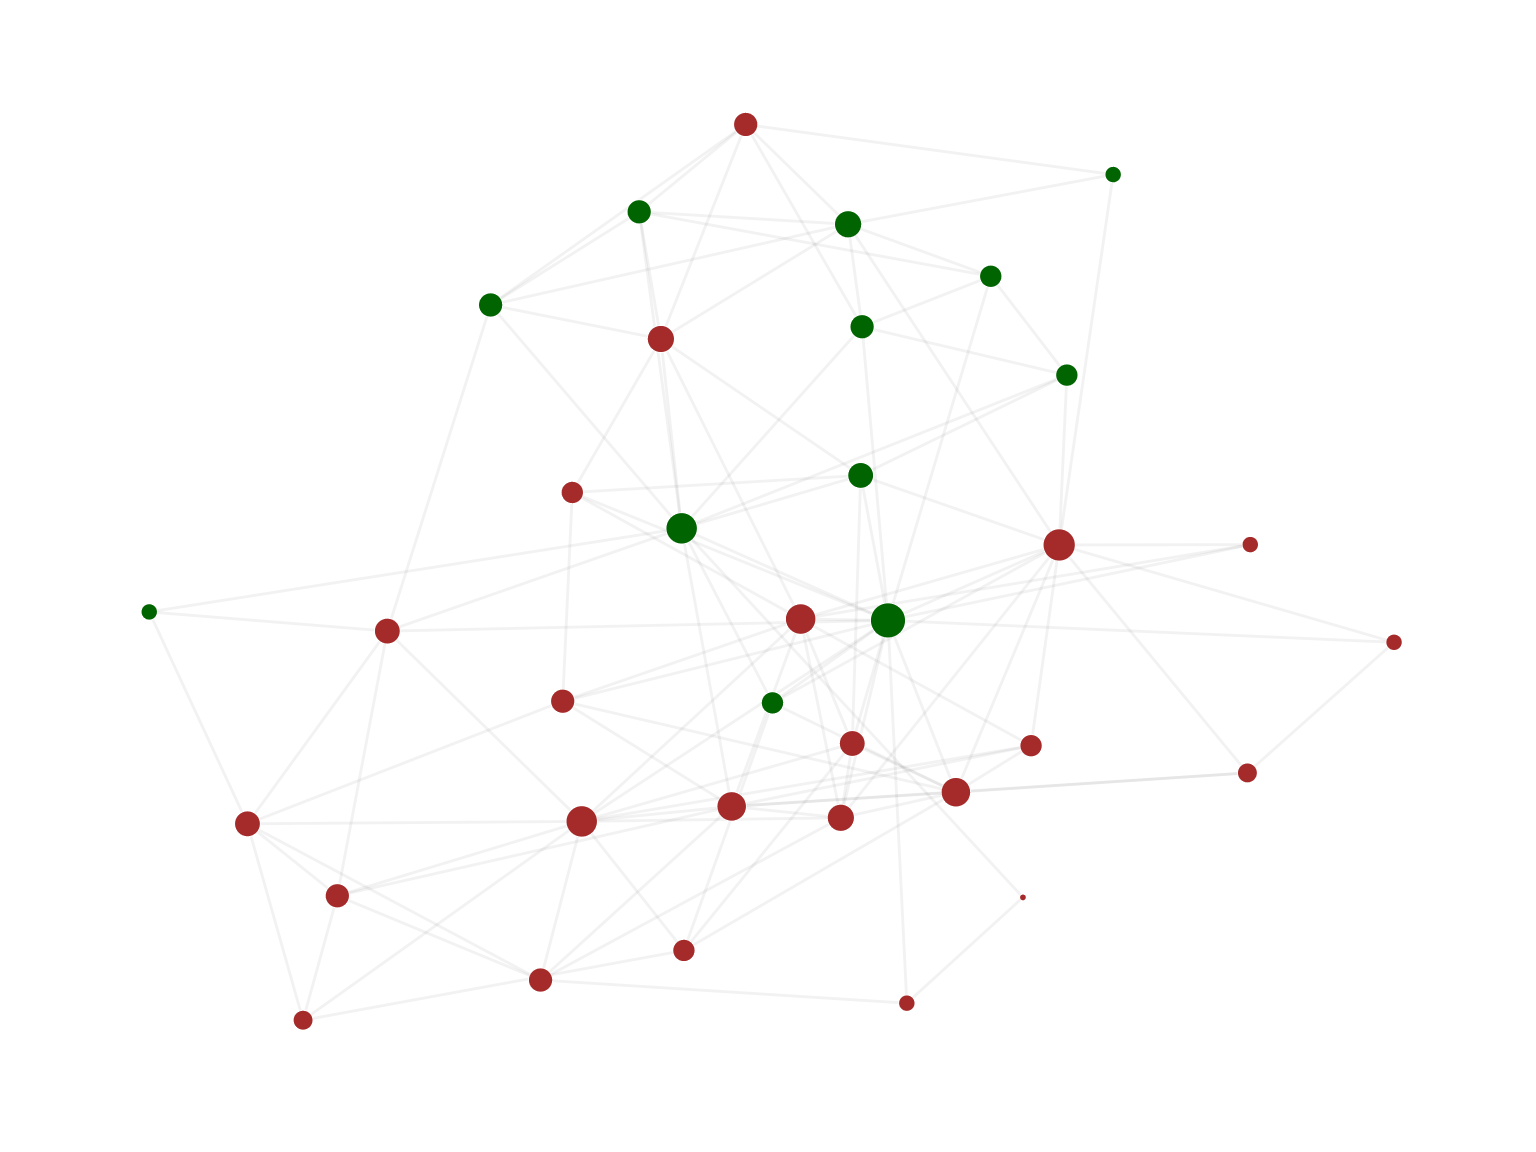
\includegraphics[width=.9\textwidth]{overview/mexican_elites-1}
\end{frame}

{%<--- Start local changes
\setbeamertemplate{navigation symbols}{}
\usebackgroundtemplate{
    \hspace{-1em}
    
\includegraphics[width=1.03\paperwidth]{thats-all-folks}
}
\begin{frame}{Thank you! Questions?}
\hfill
\begin{minipage}{.65\textwidth}
    \vspace{14.4em}
    \begin{tcolorbox}[
        width=1.1\textwidth,
        colback=black!5,
        title=\textbf{Contact}
    ]
    \texttt{\scriptsize{
        \hspace{-1.2em}
        \faIcon{envelope}\enspace
        \textcolor{blue}{\href{mailto:stalaga@uw.edu.pl}{stalaga@uw.edu.pl}} \\
        \faIcon{address-card}
        \href{http://iss.uw.edu.pl/en/szymon-talaga/}{iss.uw.edu.pl/en/szymon-talaga}
    }}
    \end{tcolorbox}
\end{minipage}
\end{frame}
}%<---- Finish local changes


\end{document}
